\chapter{Anexo C}
\label{cap:AnexoC}

A continuación se muestra el cuestionario que se realizó para la prueba de usabilidad.
Se muestran primero todas las preguntas (figuras \ref{Fig:pregunta_1} - \ref{Fig:pregunta_10}), y luego sus respuestas (figuras \ref{Fig:cuestionario_1} - \ref{Fig:cuestionario_10}).

\begin{figure}[h]
\centering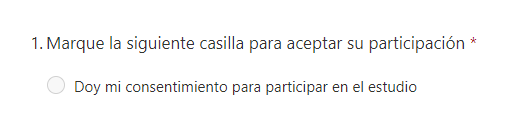
\includegraphics[width=0.5\linewidth]{figs/pregunta_1.png}
\caption{Pregunta 1 del cuestionario.}
\label{Fig:pregunta_1}
\end{figure}

\begin{figure}[h]
\centering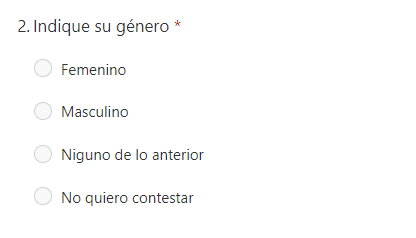
\includegraphics[width=0.5\linewidth]{figs/pregunta_2.png}
\caption{Pregunta 2 del cuestionario.}
\label{Fig:pregunta_2}
\end{figure}

\begin{figure}[h]
\centering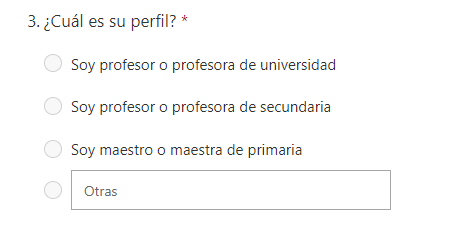
\includegraphics[width=0.5\linewidth]{figs/pregunta_3.png}
\caption{Pregunta 3 del cuestionario.}
\label{Fig:pregunta_3}
\end{figure}

\begin{figure}[h]
\centering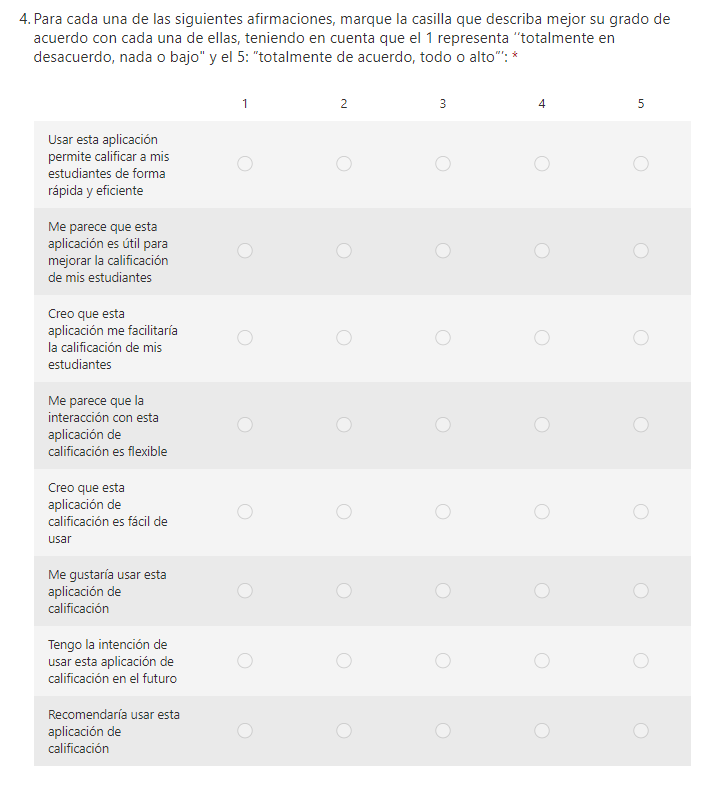
\includegraphics[width=1\linewidth]{figs/pregunta_4.png}
\caption{Pregunta 4 del cuestionario.}
\label{Fig:pregunta_4}
\end{figure}

\begin{figure}[h]
\centering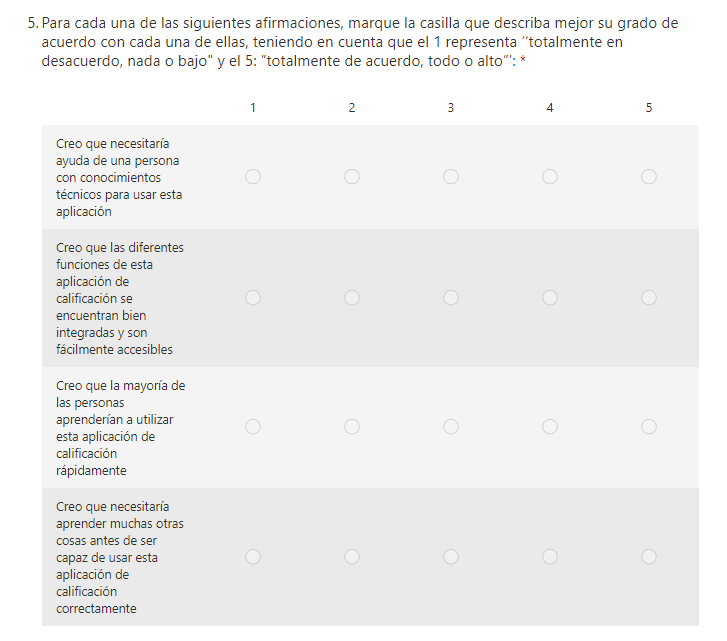
\includegraphics[width=1\linewidth]{figs/pregunta_5.png}
\caption{Pregunta 5 del cuestionario.}
\label{Fig:pregunta_5}
\end{figure}

\begin{figure}[h]
\centering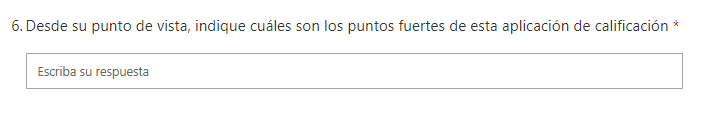
\includegraphics[width=0.5\linewidth]{figs/pregunta_6.png}
\caption{Pregunta 6 del cuestionario.}
\label{Fig:pregunta_6}
\end{figure}

\begin{figure}[h]
\centering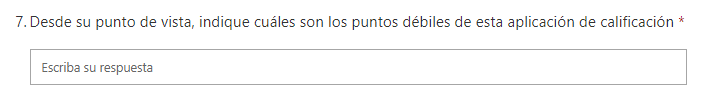
\includegraphics[width=0.5\linewidth]{figs/pregunta_7.png}
\caption{Pregunta 7 del cuestionario.}
\label{Fig:pregunta_7}
\end{figure}

\begin{figure}[h]
\centering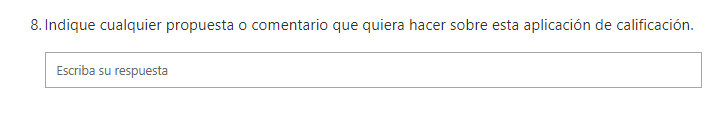
\includegraphics[width=0.5\linewidth]{figs/pregunta_8.png}
\caption{Pregunta 8 del cuestionario.}
\label{Fig:pregunta_8}
\end{figure}

\begin{figure}[h]
\centering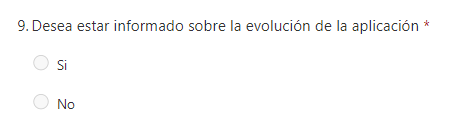
\includegraphics[width=0.5\linewidth]{figs/pregunta_9.png}
\caption{Pregunta 9 del cuestionario.}
\label{Fig:pregunta_9}
\end{figure}

\begin{figure}[h]
\centering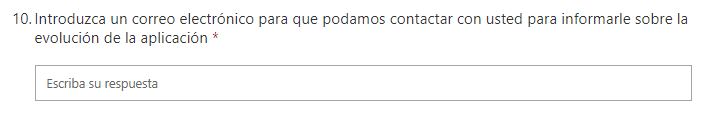
\includegraphics[width=1\linewidth]{figs/pregunta_10.png}
\caption{Pregunta 10 del cuestionario.}
\label{Fig:pregunta_10}
\end{figure}

\begin{figure}[h]
\centering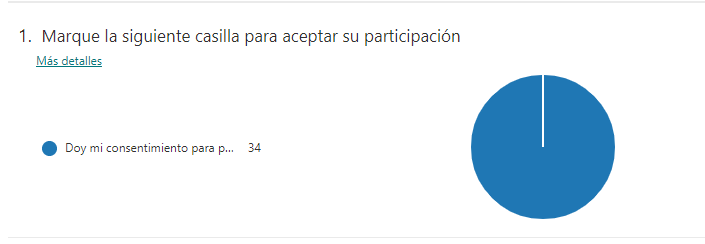
\includegraphics[width=1\linewidth]{figs/cuestionario_1.png}
\caption{Respuestas a la pregunta 1 del cuestionario.}
\label{Fig:cuestionario_1}
\end{figure}

\begin{figure}[h]
\centering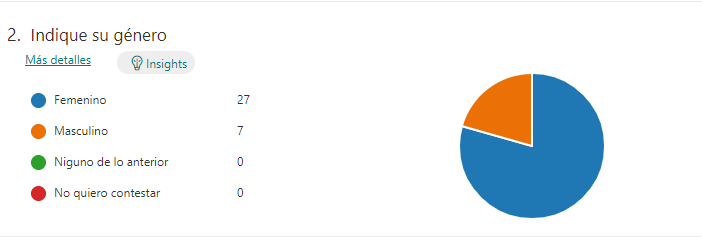
\includegraphics[width=1\linewidth]{figs/cuestionario_2.png}
\caption{Respuestas a la pregunta 2 del cuestionario.}
\label{Fig:cuestionario_2}
\end{figure}

\begin{figure}[h]
\centering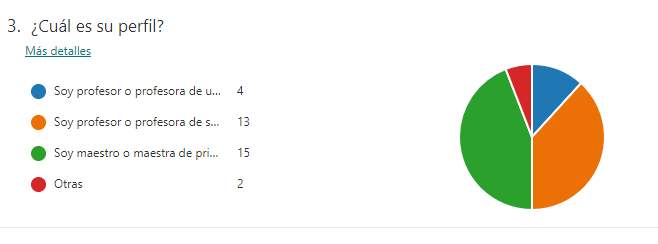
\includegraphics[width=1\linewidth]{figs/cuestionario_3.png}
\caption{Respuestas a la pregunta 3 del cuestionario.}
\label{Fig:cuestionario_3}
\end{figure}

\begin{figure}[h]
\centering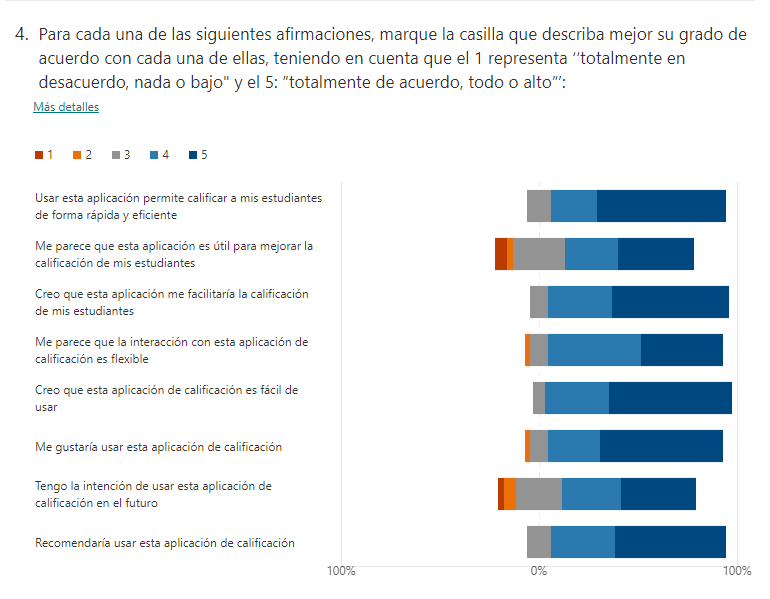
\includegraphics[width=1\linewidth]{figs/cuestionario_4.png}
\caption{Respuestas a la pregunta 4 del cuestionario.}
\label{Fig:cuestionario_4}
\end{figure}

\begin{figure}[h]
\centering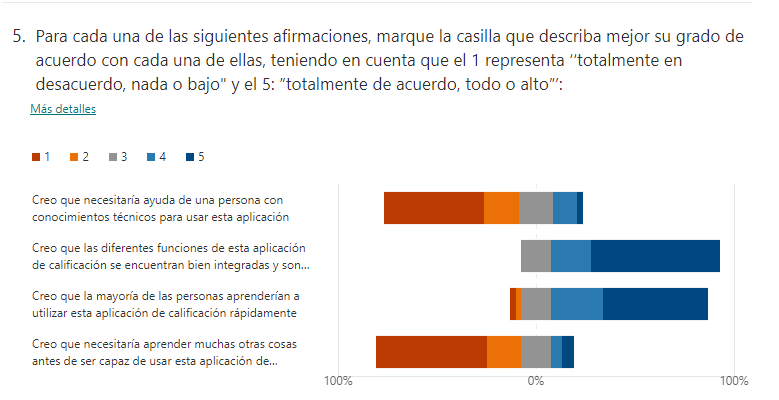
\includegraphics[width=1\linewidth]{figs/cuestionario_5.png}
\caption{Respuestas a la pregunta 5 del cuestionario.}
\label{Fig:cuestionario_5}
\end{figure}

\begin{figure}[h]
\centering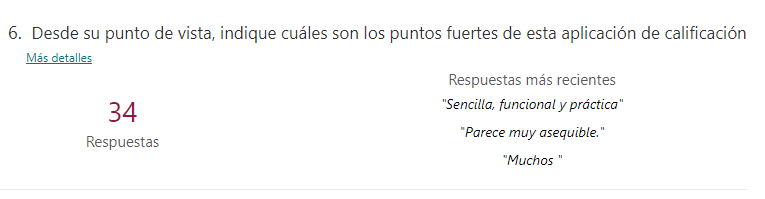
\includegraphics[width=1\linewidth]{figs/cuestionario_6.png}
\caption{Respuestas a la pregunta 6 del cuestionario.}
\label{Fig:cuestionario_6}
\end{figure}

\begin{figure}[h]
\centering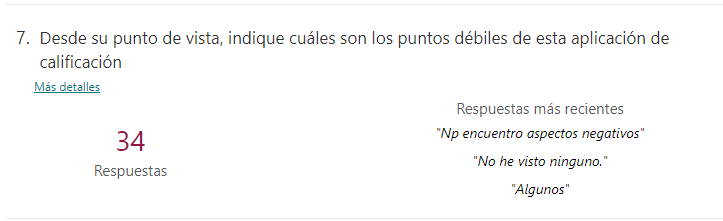
\includegraphics[width=1\linewidth]{figs/cuestionario_7.png}
\caption{Respuestas a la pregunta 7 del cuestionario.}
\label{Fig:cuestionario_7}
\end{figure}

\begin{figure}[h]
\centering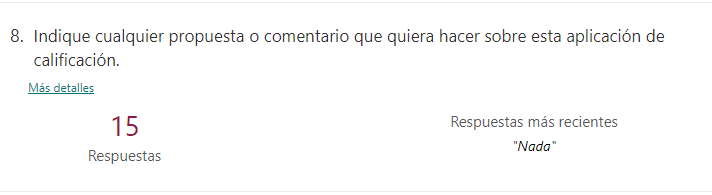
\includegraphics[width=1\linewidth]{figs/cuestionario_8.png}
\caption{Respuestas a la pregunta 8 del cuestionario.}
\label{Fig:cuestionario_8}
\end{figure}

\begin{figure}[h]
\centering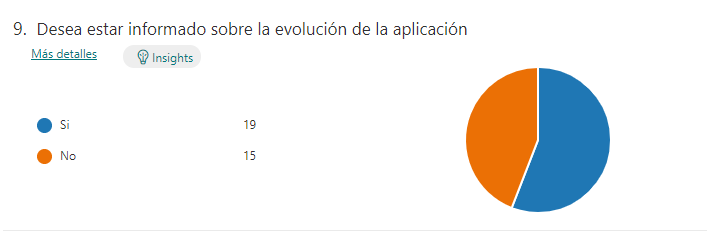
\includegraphics[width=1\linewidth]{figs/cuestionario_9.png}
\caption{Respuestas a la pregunta 9 del cuestionario.}
\label{Fig:cuestionario_9}
\end{figure}

\begin{figure}[h]
\centering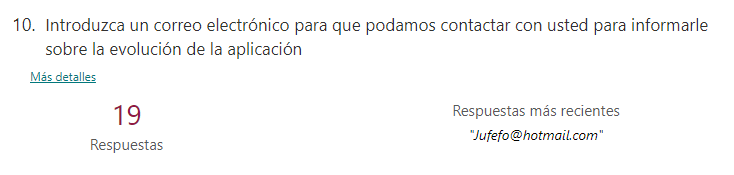
\includegraphics[width=1\linewidth]{figs/cuestionario_10.png}
\caption{Respuestas a la pregunta 10 del cuestionario.}
\label{Fig:cuestionario_10}
\end{figure}